%% ================================================================
%% # DBIS Databases Data Analysis Project Part 0 Template
%% 
%% Template for students to hand-in their databases exercise solutions.
%% 
%% [Databases and Information Systems Group](https://dbis.dmi.unibas.ch/)
%%
%% ## Usage
%% 
%% Fill in the required fields and write your submission
%%
%% ## Issues
%%
%% See dbisdbprojp0.sty for further information.
%% ================================================================
\documentclass{article}
\usepackage{dbisdbprojp0}
\usepackage{url}
\usepackage{float}



%% ================================================================
%%
%% General Information
%%
%% ================================================================
%%
%% Add your information here
\course       {Databases}
\semester     {Autumn 2020}
\title        {Data Analysis Project\\P2: Data Integration}
\subtitle     {Visualizing Traffic density data and comparing them to air pollution- and meteorological data in Basel, London and Los Angeles}
\studenta     {Pascal Kunz}
\studentb     {Etienne Mettaz}
%\studentc     {Alan Turing}


%% ================================================================
%%
%% Common Packages
%%
%% ================================================================
%%
%% Useful common packages for this course

%% Drawing everything, with lots of libraries
\usepackage{tikz}
%% A library providing ER prefabs
\usetikzlibrary{er}

%% ================================================================
%%
%% Custom Packages
%%
%% ================================================================
%%
%% Add custom packages below:
%%


\begin{document}
%% Required for the title
\printfront
%% ================================================================
%%
%% Description
%%
%% ================================================================


\newpage

\section{Updated ER-Diagram}

This section present the current ER Diagramms of the integrated data.
\begin{figure}[H]
\centering
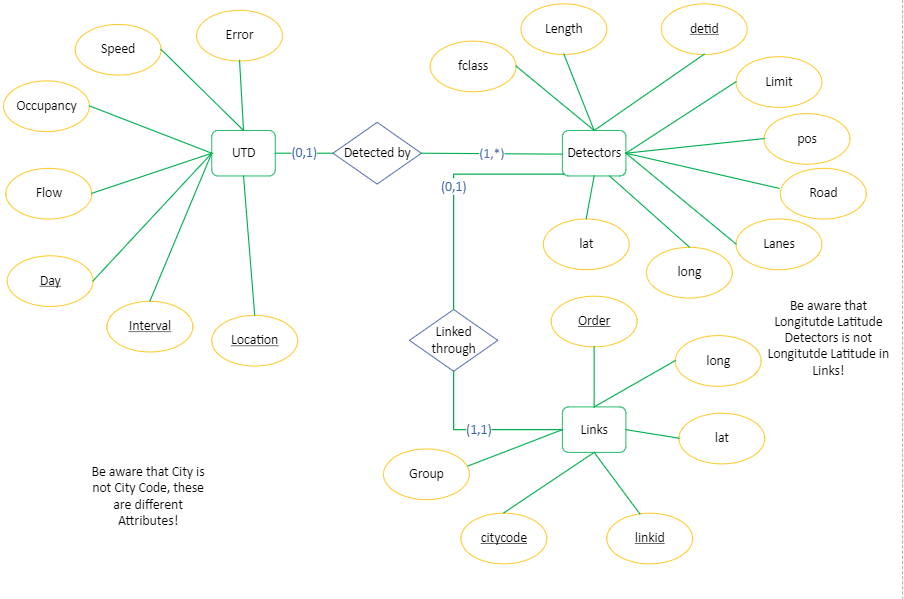
\includegraphics[width=11cm]{first.png}
\caption{ER Diagramm of the utd19 traffic data}
\end{figure}

\begin{figure}[H]
\centering
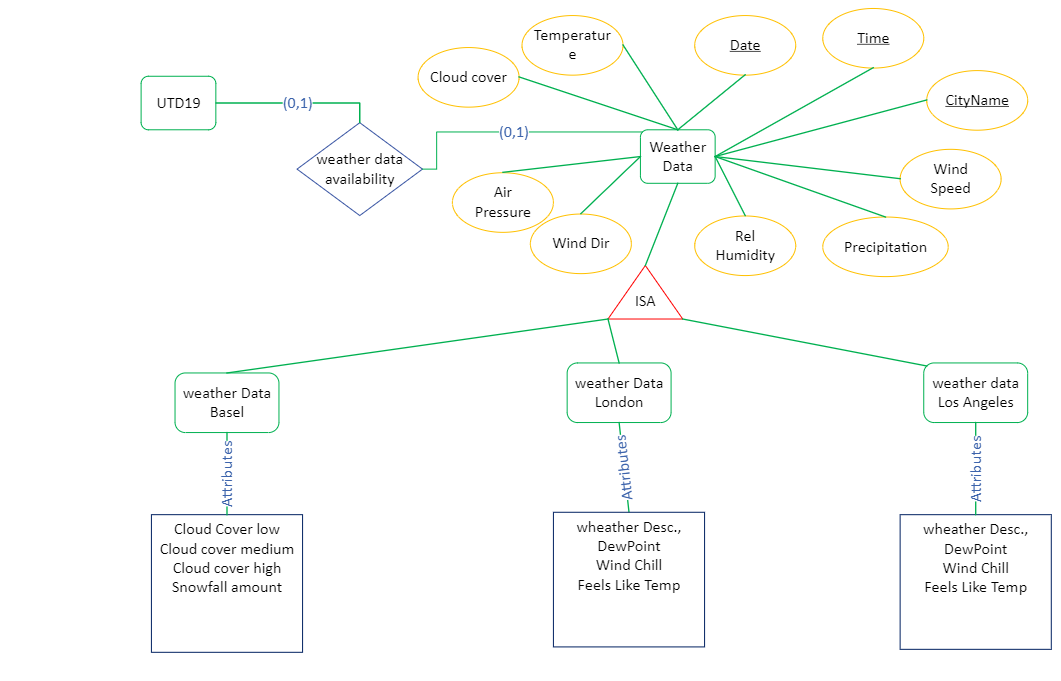
\includegraphics[width=11cm]{second.png}
\caption{ER Diagramm of the weather datas. All attributes are written in a box for ease of read}
\end{figure}

\begin{figure}[H]
\centering
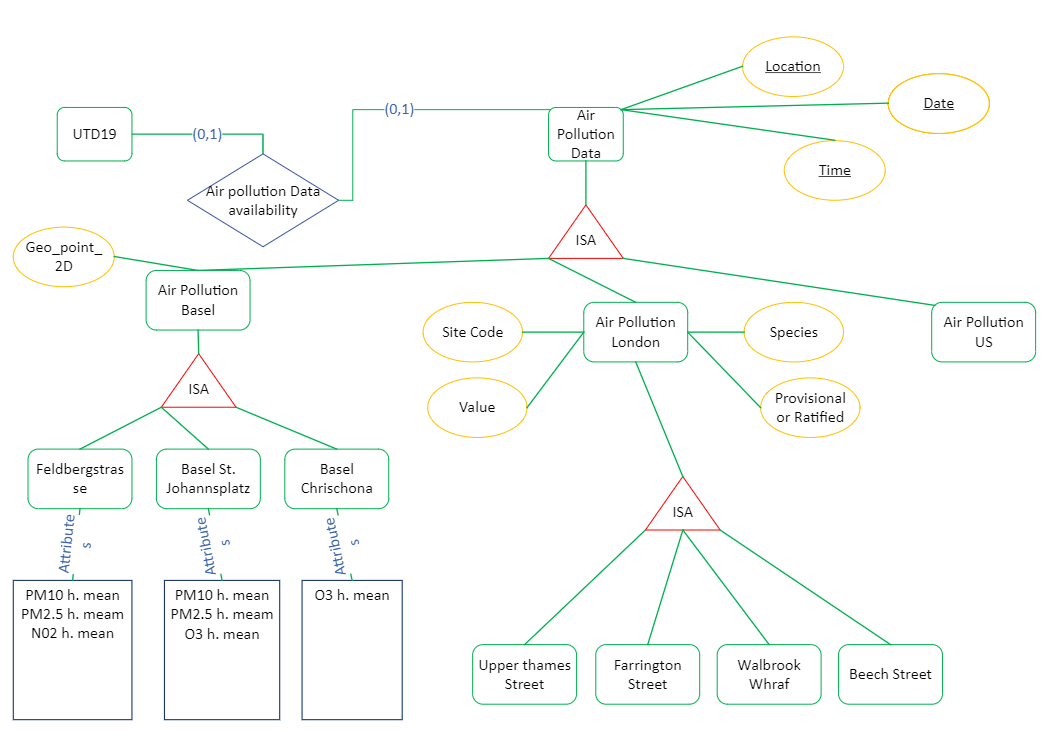
\includegraphics[width=11cm]{third.png}
\caption{ER Diagramm of the air pollution datas. All attributes are written in a box for ease of read}
\end{figure}

\begin{figure}[H]
\centering
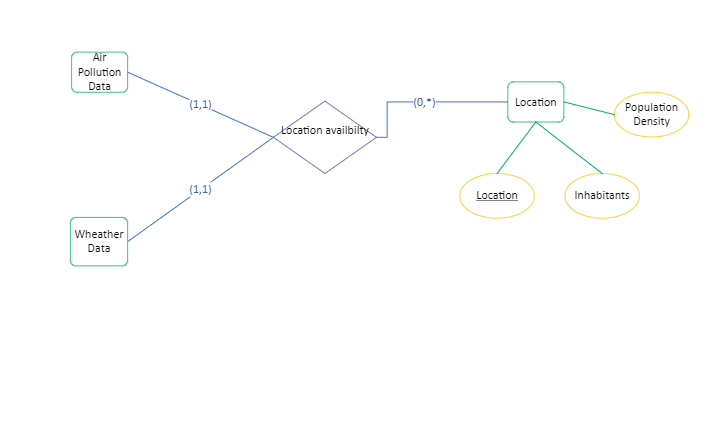
\includegraphics[width=11cm]{fourth.png}
\caption{ER Diagramm of the location data}
\end{figure}

\begin{figure}[H]
\centering
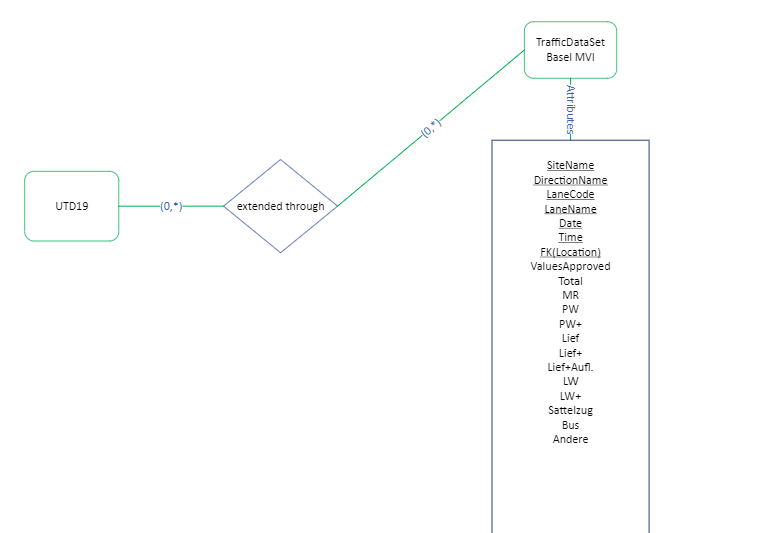
\includegraphics[width=11cm]{fifth.png}
\caption{ER Diagramm of an additional traffic data source}
\end{figure}


%%%%%%%%%%%%%%%%%%%%%%%%%%%%%%%%%%%%%%%%%%%%%%%%%%%%
%%%%%%%%%%%%%%%%%%%%%%%%%%%%%%%%%%%%%%%%%%%%%%%%%%%%
\section{Updated logical scheme}
\begin{center}
\begin{tabbing}
    UTD19 \qquad\qquad\qquad\= (\uline{Date, Interval, \uwave{DetID}}, \uwave{Location}, Flow, Occupancy, Speed)\\
    
    Detectors \> (\uline{{DetID}, \uwave{City Code}}, Length, Road,  Limit, Position, Lanes,\\ \> Longitude, Latitude, fclass, Road)\\

    Links \> (\uline{LinkID, City Code},  \uwave{DetID}, Order, Latitude, Longitude, Group)\\\\\\
    

    
    % Do we need CityName ? (already Location)
    Weather Data \> (\uline{Date, Time},  \uwave{Location}, Temperature, Wind Speed, Precipitation,\\ \> Rel Humidity, Wind Direction, Air pressure, Cloud Coverage)\\\\\\% Snowfall amount

  
    
% Ich bin nicht sicher, dass wir ``Provisional or Ratified'' brauchen
% Wir müssen sicher stellen, das die Ordnung der Pollutant consistant ist
    Air Pollution Data \> (\uline{Date, Time, Site Code}, \uwave{Location},  Species\\ \> Latitude, Longitude, Value)\\\\\\
    
    
   % Ich bin mit keys nicht sicher
    Basel MVI \> (\uline{\uwave{Location}, Time, Day, SiteName, DirectionName, LaneCode}, LaneName, Date,\\ \> TimeFrom, Time To, DateTimeFrom, DateTimeTo, Year, ValuesApproved,\\ \> ValuesEdited, Total, MR, PW, PW+, Lief, Lief+, Lief+Aufl., LW, LW+,\\ \> Sattelzug, Bus, Andere )\\\\\\
    
    Location \> (\uline{Location}, Inhabitants, Population Density)
    
\end{tabbing}    
\end{center}

\section{Guide to replay the integration}

We have decided to do the DataCleaning with Python using Pandas. Therefore we have created three folder with Code under p2// DataCleaning.

\subsection{Weather Cleaning}

The Weather Cleaning consists of four main files: 1 for each City and one file to unify them. The Datacleaning is done by running the four main functions of the respective files.

\subsection{Air Pollution cleaning}
The Air Pollution cleaning consists of five main files: 1 for each City, 1 for  a Dictionary of Pollutant values and 1 file to unify them. The cleaned output files are being produced by running the four main functions of the respective files.

\subsection{Traffic Cleaning}
The Traffic Cleaning consists of three main files: the cleaning for the UTD Dataset, for the Basel MIV Dataset as well as for the links of the UTD Dataset. The cleaned output files are being produced by running the respective main functions.

\subsection{Integration Code}
Upon setting up the database, we can fill the schemes by running this code:

\lstinputlisting[language=sql]{Dataloader.sql}


\end{document}
